\newpage
\chapter{Platform}
\section{Environment}
The system is primarily to be used from the same PC, as the webpage is part of an energy system
placed at the school AU Herning. A part of the energy system is a screen showing the webpage to
be able to control the system nearby it. The screens resolution is 1024x768 pixels (fullscreen with no system bars or dock), 
which is the size the site has been optimized for. Also the website has been optimized for small-screen devises with a resolution from 350x480 pixels (as this resolution has been used for several phones in the last years).
\section{File Structuer}
The website can be seen on http://www.ehub.threee.dk/, the file structure on the ftp server is as follow. In the index folder/root of the site, the folders: Design, Images, Scripts and Modules can be found together with the different .html files and .css files created for the main design of the page. The folders contains:
\begin{itemize}
	\item Design: Photoshop files
	\item Images: Icons and other pictures used on the site.
	\item Scripts: Java-scripts used
	\item Modules: All html and css files used inside the frames in the module pages.
\end{itemize}
Inside the Modules folder, a folder is created containing the files used by each module (wind turbine, battery, caes, photovoltaic cells). Later it is explained how this is implemented in the code and why the folder setup is made like this.
\begin{figure}[htbp]
	\center
	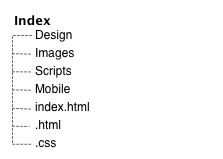
\includegraphics[width=0.3\textwidth]{images/hierarki.png} % requires the graphic package
   	\caption{Hierarki of the files}
   	\label{fig:file_hierarki}
\end{figure}

